\documentclass[12pt]{article}

\usepackage{amsmath}
\usepackage{graphicx}
\usepackage{hyperref}
\usepackage[margin=1.2in]{geometry}

\newenvironment{myitemize}
{ \begin{itemize}
    \setlength{\itemsep}{0pt}
    \setlength{\parskip}{0pt}
    \setlength{\parsep}{0pt}     }
{ \end{itemize}                  } 

\providecommand{\eqn}[1]{eqn.~(\ref{eqn:#1})}
\providecommand{\tab}[1]{Table~\ref{tab:#1}}
\providecommand{\fig}[1]{Figure~\ref{fig:#1}}

\providecommand{\vecsymbol}[1]{\ensuremath{\boldsymbol{#1}}}
\providecommand{\pv}{\vecsymbol{p}}
\providecommand{\deltav}{\vecsymbol{\delta}}

\title{Tech Note on Quality Assurance for DESI Spectroscopic Reduction \\
\vspace{5mm}{\large\bf DESI-doc-XXX-v1.1}}
\author{J. Xavier Prochaska, Govinda Dhungana}

\begin{document}
\maketitle

\section{Introduction}

This technical note is intended to summarize 
the Quality Assurance (QA) outputs for the
{\tt desispec} package, including both the full (offline)
spectroscopic pipeline and the Quicklook pipeline 
(run on mountain).  It is a living document, to be
updated as algorithms and outputs evolve.

This document is currently
maintained in the {\tt desispec} 
package\footnote{Maintained in the public github repository at \url{https://github.com/desihub/desispec}} under {\tt doc/tex/}
and is also summarized on the DESI Wiki at 
\url{https://desi.lbl.gov/trac/wiki/Pipeline/QualityAssurance}. 
This document supersedes the Wiki.

\section{General Architecture}

A basic framework for controlling and packaging
QA analysis is provided in the
{\tt qa\_exposure.py} module
within {\tt desispec/py/qa/}.
This includes defining parameters that guide the QA
algorithms, set thresholds for raising warnings, etc.
All QA plotting codes will be kept within the separate
module {\tt qa\_plots.py} in the same folder.

The QA analysis is performed as part of the scripts for each
of the primary spectroscopic pipeline steps (e.g.\ fiberflat,
sky subtraction, fluxing).   The QA algorithms are located 
within the modules that perform each step (e.g.\ {\tt sky.py}).
These evaluate a set of QA metrics that are stored
in a QA dict.

To allow for multi-processing the QA metrics are stored
on the hard-drive in a set of YAML files, one per frame.
The naming convention for the QA frame files 
will be
{\tt qa}-{\tt spectrograph}-{\tt exposure}.yaml or
e.g. {\tt qa-b0-00000002.yaml}.
If multiple QA diagnostics are generated for a given
frame (e.g. sky subtraction and flux calibration for
a science frame), then the YAML file is updated 
at each step.
It is likely that these YAML files will be collated
once the processing of all frames for 
a given exposure is complete
[not yet implemented].


There are a set of diagnostic plots that are optionally
generated during the pipeline steps.  It is not likely that
these will be created during routine operation of the
pipeline.
Currently most (but not all)
of the plots can be generated
from the standard files produced by the pipeline steps.  
The team will likely write the additional data to 
hard-drive so that all of the plots can be made without
running the full pipeline. 
The plots are currently written as PDF but an alternate
framework can easily be implemented.
The current naming convention includes the type
of QA in the filename, e.g.
{\tt qa}-{\tt sky}-{\tt spectrograph}-{\tt exposure}.pdf. 

A primary role of the QA analysis is to identify
data that is significantly inconsistent with 
expectation, e.g.\ too high of a bias level in 
a specific detector, insufficient flux in the
flat field frames.  To enable these tests, 
a set of reference data must be provided.
We foresee these data being ingested from a set
of YAML and FITS files distributed with the
{\tt desispec} pipeline 
[not yet implemented].
These data will need, of course, to be updated
as the instrument and/or software evolves.
In addition, we may implement a warning system
(beyond the standard logging) to notify personnel
when specific QA metrics are far from nominal
[not yet implemented].



\section{Pre-Processing}

[not yet implemented]

QA will be generated to assess the meta data
of the raw data files, the success/failure of 
the pipeline to link science frames to calibration
frames, and any other critical activities prior
to image processing.

\section{Image Processing}

[not yet implemented]

QA will be generated to examine the basic
image quality.  The image sizes, detector
bias levels, incidence of cosmic rays will
all be monitored and checked against reference
values.

\section{PSF}

[not yet implemented]

The fits to the point spread function (PSF)
and wavelength calibration will be assessed
and compared against reference values.
Significant deviations between fibers will
be assessed.     

%This section will describe the QA related to
%point spread function (PSF) evaluation, 
%wavelength calibration, and extraction.

\section{Flat Fielding}

\subsection{Overview}

The primary goals of QA related to flat fielding are:

\begin{myitemize}
\item Crudely assess system throughput (i.e.\ sufficient counts)
\item Assess flat field variation in fibers
\item Identify bad fibers
\item Assess flat field within a frame (wedge) 
\item Assess flat field throughout an exposure
\item Assess flat field versus time
\end{myitemize}

\subsection{Single Frame}

The {\tt desi\_compute\_fiberflat} routine calculates a 
deconvolved, mean fiber spectrum from all of the fibers in a given 
flat field frame. 
The routine then calculates (and saves) a fiberflat spectrum for each 
fiber. This is the fiber's flux normalized by the mean spectrum 
and convolved with the fiber's resolution.  
These fiberflat spectra
may then be used to correct for pixel-to-pixel variations 
and a mean offset.

The fiberflat QA analysis on a single flat field frame 
is guided by the set of
parameters defined in {\tt qa\_exposure.QA\_Frame.init\_fiberflat}.
These parameters are primarily used 
to raise warnings if the QA metrics exceed the parameter values.
Table~\ref{tab:flat_param} summarizes the parameters.

\begin{table}[h]
\begin{center}
\caption{Fiberflat QA Parameters}
\label{tab:flat_param}
\begin{tabular}{p{3.5cm}p{1.2cm}p{8.3cm}}
\hline
{\bf Name} & {\bf Value} & {\bf Brief Description}\\
\hline
MAX\_N\_MASK    & 20000 & Maximum allowed number of pixels masked in fit \\
MAX\_SCALE\_OFF & 0.05  & Maximum allowed fractional offset between mean spectrum and individual fiber flux \\ 
MAX\_OFF        & 0.15  & Maximum allowed offset from unity for any pixel in the fiberflat spectra\\
MAX\_MEAN\_OFF  & 0.05  & Maximum allowed offset from unity for the mean of any fiberflat \\
MAX\_RMS        & 0.02  & Maximum allowed RMS in any fiberflat (off unity) \\
\hline
\end{tabular}
\end{center}
\end{table}



\subsubsection{Metrics}

Table~\ref{tab:flat_metrics} summarizes the QA metrics measured
for the fiberflat step.  

\begin{table}[h]
\begin{center}
\caption{Fiberflat QA Metrics}
\label{tab:flat_metrics}
\begin{tabular}{p{3.5cm}p{9.0cm}}
\hline
{\bf Name} & {\bf Brief Description}\\
\hline
MAX\_MEANSPEC   & Maximum flux (counts) in the mean fiber flat spectrum \\ 
CHI2PDF         & Reduced $\chi^2$ for fit to mean spectrum \\
N\_MASK         & Number of pixels masked in fit (all fibers) \\
MAX\_SCALE\_OFF & Maximum difference between the ratio of the fiber flux and 
  the mean spectrum \\
MAX\_OFF        & Maximum offset from unity in all of the fiberflats \\
MAX\_MEAN\_OFF  & Maximum offset from unity for the mean of all fiberflats \\
MAX\_RMS        & Maximum RMS in the fiberflats (from unity) \\
\hline
\end{tabular}
\end{center}
\end{table}


\noindent
Here is a summary of each:

\vskip 0.2in

\noindent
{\tt MAX\_MEANSPEC}:  Peak flux in the mean fiber flat spectrum 
(counts).  Assesses system throughput and flat field lamp.

\noindent
{\tt CHI2PDF}:  This metric records the reduced $\chi^2$ value 
for the fit that generated the mean spectrum.

\noindent
{\tt N\_MASK}:  This metric records the number of pixels that were
masked during the fiberflat fit.  It is the sum over all fibers.

\noindent
{\tt MAX\_SCALE\_OFF}:  This metric records the maximum offset 
in the ratio of the flux in each fiber to the mean spectrum.
The median ratio of flux/mean
is calculated for each fiber and the maximum
deviation from unity is recorded together with the fiber number.  
This metric is useful for
identifying whether one (or more) fibers have abnormal flux.

\noindent
{\tt MAX\_OFF}:  This metric records the maximum offset from
unity for all the fiberflats at all pixels.
This may identify if one or more fibers have abnormal response.

\noindent
{\tt MAX\_MEAN\_OFF}:  This metric records the maximum offset from
unity of the mean of each of the fiberflats together with the
fiber number.  May also be used
to identify one or more fibers with abnormal response.

\noindent
{\tt MAX\_RMS}:  This metric records the maximum RMS amongst
all the fiberflats (relative to unity) and the fiber number.

\subsubsection{Figure(s)}

A series of plots of the fiber flux, mean of the fiberflat, and
RMS in the fiberflats are shown in each tile.
These are most useful for identifying outlier flat field
fibers in a given frame, but also to identify gradients 
in the flat field flux.

\begin{figure}[htb]
\begin{center}
\includegraphics[width=5in]{fig/qa-flat}
\caption{Example figure of fiberflat QA
for a single frame.  
}
\label{fig:fiberflat_frame}
\end{center}
\end{figure}


\subsection{Exposure}

QA code will be written to:

\begin{myitemize}
\item Compare the mean spectra across an exposure (per camera)
\item Compare the CHI2PDF across an exposure (per camera)
\item Assess the RMS in the fiberflats across an exposure (per camera)
\end{myitemize}

\subsection{Time}

QA code will be written to:

\begin{myitemize}
\item Assess the flat field flux with time
\item Assess the CHI2PDF values with time
\item Assess the RMS in the fiberflats with time
\end{myitemize}

%%%%%%%%%%%%%%%%
\section{Sky Subtraction}

\subsection{Overview}

The primary goals of QA for sky subtraction are to:

\begin{myitemize}
\item Assess residuals (global)
\item Assess residuals (on sky lines)
\item Identify bad sky fibers
\item Examine performance within an exposure
\item Examine performance across the sky (e.g.\ tiles)
\item Examine performance vs.\ time
\end{myitemize}

\subsection{Single Frame}

The {\tt desi\_compute\_sky} method calculates a 
deconvolved sky model
from the set of sky fibers in a given frame.
A sky model for each fiber is then calculated from the 
mean sky model by convolving it with the fiber resolution.

The sky subtraction QA analysis on a single 
frame examines the residuals of sky-subtracted flux in each sky fiber
and the $\chi^2$ probability of the residuals.
If the QA metrics exceed the 
parameter values listed in Table~\ref{tab:sky_param},
warnings are raised.

\begin{table}[h]
\begin{center}
\caption{Sky Subtraction QA Parameters}
\label{tab:sky_param}
\begin{tabular}{p{3.5cm}p{1.2cm}p{8.3cm}}
\hline
{\bf Name} & {\bf Value} & {\bf Brief Description}\\
\hline
PCHI\_RESID    & 0.05 & Minimum $P(\chi^2)$ allowed for sky fiber residuals \\ 
PER\_RESID     & 95   & Percentile value for residual distribution calculation\\
\hline
\end{tabular}
\end{center}
\end{table}

\subsubsection{Metrics}

Table~\ref{tab:sky_metrics} summarizes the QA metrics measured
for the sky subtraction step.  

\begin{table}[h]
\begin{center}
\caption{Sky Subtraction QA Metrics}
\label{tab:sky_metrics}
\begin{tabular}{p{4.3cm}p{9.0cm}}
\hline
{\bf Name} & {\bf Brief Description}\\
\hline
NSKY\_FIBER           & Number of sky fibers in the frame \\
NREJ                  & Number of pixels rejected in sky model fit \\
NBAD\_PCHI            & Number of sky fibers with $P(\chi^2) < $PCHI\_RESID \\
MED\_RESID            & Median residuals from all sky fibers \\
RESID\_PER            & Percentiles of residuals from all sky fibers \\
MED\_SKYLINE\_RESID   & Median residuals on sky lines from all sky fibers [not yet implemented]\\
\hline
\end{tabular}
\end{center}
\end{table}


\noindent
Here is a summary of each:

\vskip 0.2in

\noindent
{\tt NSKY\_FIBER}:  Records the number of sky fibers in the frame.

\noindent
{\tt NBAD\_PCHI}:  Records the number of sky fibers with a 
$\chi^2$ probability in the residuals less than PCHI\_RESID.  
Variance in the sky model is included.
A warning is thrown if NBAD\_PCHI~$>0$.

\noindent
{\tt MED\_RESID}:  Median of the residuals of the sky-subtracted
sky fibers.  Ideally, this will be very close to 0.

\noindent
{\tt RESID\_PER}:  Percentile residual values corresponding to the
PER\_RESID parameter for the sky-subtracted sky fibers.

\subsubsection{Figure(s)}

The figure for QA on a sky-subtracted frame shows the
residuals versus wavelength and a histogram of 
the residuals relative to the estimated uncertainty. 

\begin{figure}[htb]
\begin{center}
\includegraphics[width=5in]{fig/qa-skyres}
\caption{Example figure for sky subtraction 
residual QA, for a single frame.
}
\label{fig:skysub_frame}
\end{center}
\end{figure}


\subsection{Exposure}

QA code will be written to:

\begin{myitemize}
\item Compare the sky model across tiles 
\item Compare the residuals (median and percentiles) across tiles
\item Compare the $P(\chi^2)$ values across tiles
\end{myitemize}

\subsection{Time}

QA code will be written to:

\begin{myitemize}
\item Assess the residuals with time
\end{myitemize}

%%%%%%%%%%%%%%%%
\section{Flux Calibration}

\subsection{Overview}

The primary goals of QA for flux calibration are to:

\begin{myitemize}
\item Record the zeropoint (ZP) 
\item Assess RMS in ZP
\item Identify bad standard stars
\item Examine performance across an exposure
\item Examine performance with time
\end{myitemize}

\subsection{Single Frame}

The {\tt desi\_compute\_flux\_calibration} method generates
a calibration sensitivity function.  It is derived
from the model and measured fluxes for
a set of observed standard stars ($\sim 5$ per frame).
The parameters guiding the QA analysis for flux
calibration are given in Table~\ref{tab:flux_param}.

\begin{table}[h]
\begin{center}
\caption{Flux Calibration QA Parameters}
\label{tab:flux_param}
\begin{tabular}{p{3.5cm}p{1.8cm}p{8.2cm}}
\hline
{\bf Name} & {\bf Value} & {\bf Brief Description}\\
\hline
ZP\_WAVE       & 4800/xx/xx & Wavelength for ZP evaluation (camera dependent) \\
MAX\_ZP\_OFF   & 0.2        & Maximum allowed offset in ZP for an individual standard star \\
\hline
\end{tabular}
\end{center}
\end{table}

\subsubsection{Metrics}

Table~\ref{tab:flux_metrics} summarizes the QA metrics measured
for the flux calibration step. 

\begin{table}[h]
\begin{center}
\caption{Flux Calibration QA Metrics}
\label{tab:flux_metrics}
\begin{tabular}{p{4.3cm}p{9.0cm}}
\hline
{\bf Name} & {\bf Brief Description}\\
\hline
NSTARS\_FIBER         & Number of standard star fibers in the frame \\
ZP                    & ZP of the mean calibration at ZP\_WAVE \\
RMS\_ZP               & RMS in the ZP for the set of stars\\
MAX\_ZP\_OFF          & Maximum offset in the ZP for the stars from the mean \\
\hline
\end{tabular}
\end{center}
\end{table}

\noindent
Here is a summary of each:

\vskip 0.2in

\noindent
{\tt NSTARS\_FIBER}:  Records the number of standard star fibers in the frame.

\noindent
{\tt ZP}:  Records the ZP calculated from the mean calibration.
Evaluated at the ZP\_WAVE parameter.

\noindent
{\tt RMS\_ZP}:  Records the RMS in the ZP values calculated from individual
standard stars (also at ZP\_WAVE).

\noindent
{\tt MAX\_ZP\_OFF}:  Records maximum offset between the mean ZP and the ZP
values of the individual stars.  The standard star 
fiber for the largest offset is also recorded.

\subsubsection{Plot(s)}

A plot may be generated to show the calibration function,
expressed as the ZP in AB magnitudes.
It allows a visual assessment of the throughput
and the identification of anomalous standard stars.
Figure~\ref{fig:fluxcalib_frame} shows an example.

\begin{figure}[htb]
\begin{center}
\includegraphics[width=5in]{fig/qa-fluxZP}
\caption{Example figure for flux calibration QA
for a single frame.  
}
\label{fig:fluxcalib_frame}
\end{center}
\end{figure}

%%%%%%%%%%%%%%%%
\section{Redshift Assessment}

QA code will be generated to assess the performance
of the redshift fitter in yielding precisely measured
redshifts for the targets.  
[not yet implemented]


Additional QA code exists to assess the performance
of the full pipeline when run on simulated data
(from {\tt desisim}).
The results are compared against the high-level
science requirements for the {\tt desispec} pipeline.


%\begin{figure}[htb]
%\begin{center}
%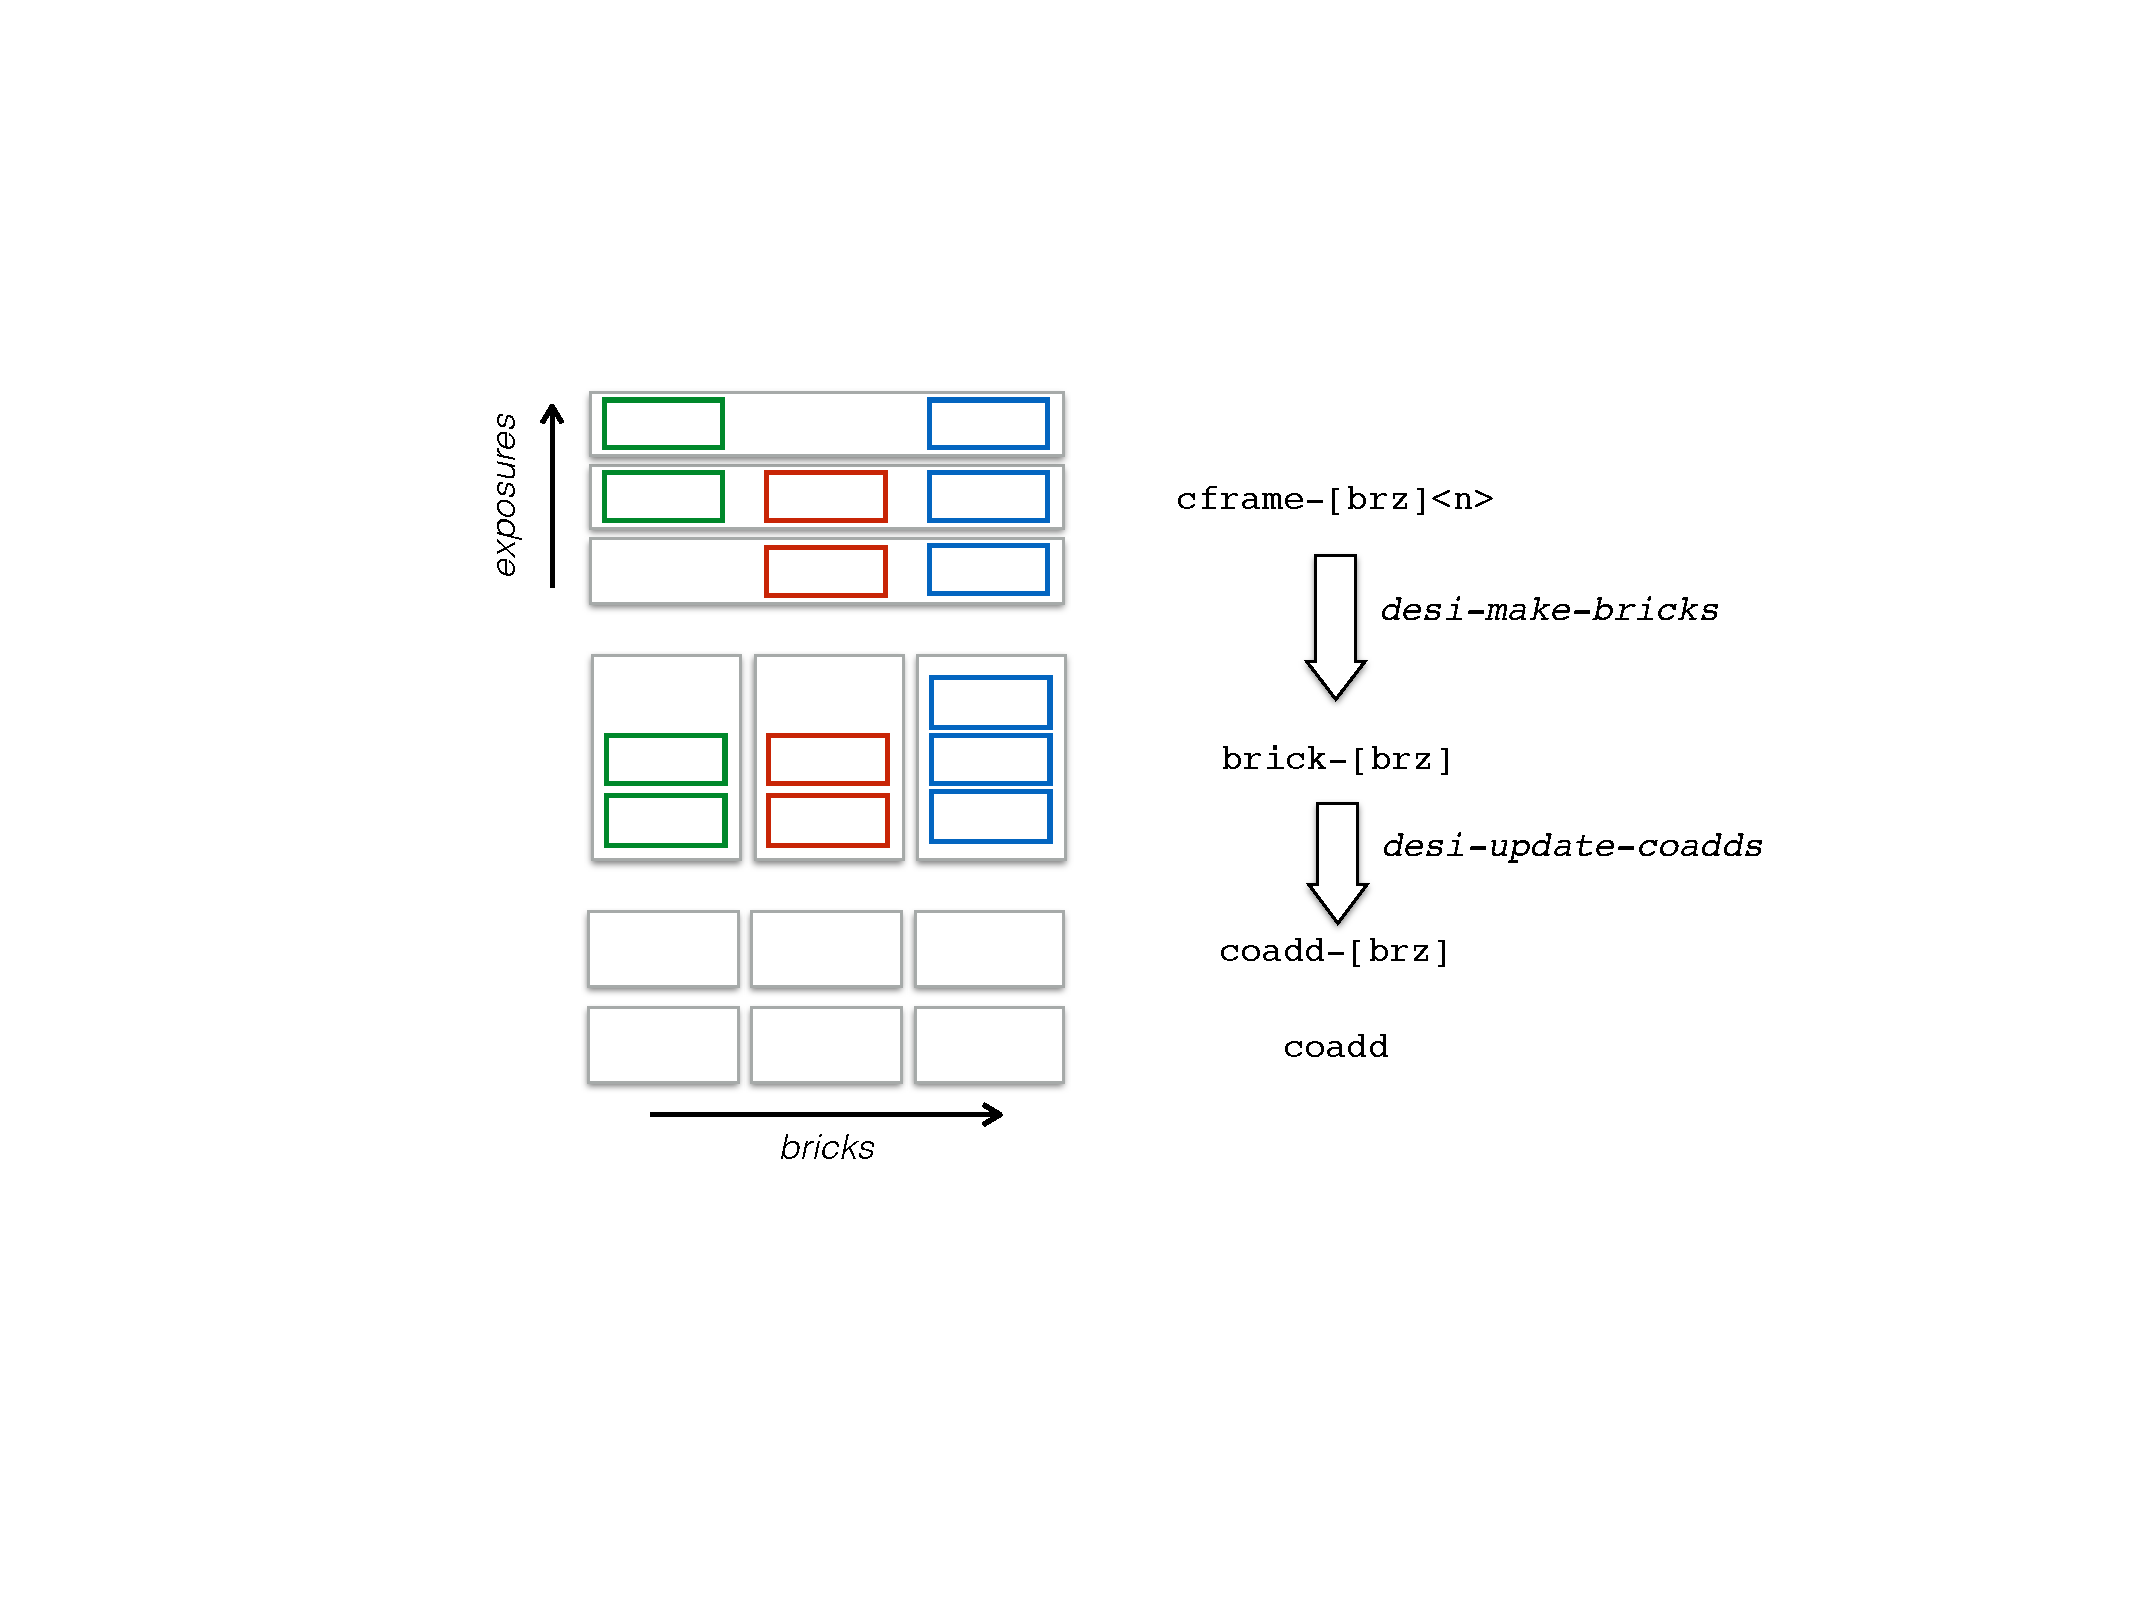
\includegraphics[width=5in]{fig/dataflow}
%\caption{Schematic representation of the coaddition dataflow. Nightly exposures are reduced to cframes (horizontal gray boxes) each covering multiple bricks (colored boxes). The {\tt desi-make-bricks} program repackages the cframe spectra into brick files (vertical gray boxes) containing all of the spectra observed for targets within a single brick. Finally, the {\tt desi-update-coadds} program reads spectra from a single brick file and generates the per-band and global coadd files (gray boxes at the bottom of the diagram).}
%\label{fig:dataflow}
%\end{center}
%\end{figure}


\def\apjl{ApJL} %Astrophysical Journal Letters
\def\aj{AJ} %Astronomical Journal
\def\apj{ApJ} %Astrophysical Journal
\def\pasp{PASP} %Publications of the Astronomical Society of the Pacific
\def\spie{SPIE} %
\def\apjs{ApJS} %Astrophysical Journal Supplement
\def\araa{ARAA} %Annual Review of Astronomy and Astrophysics
\def\aap{A\&A} %Astronomy and Astrophysics
\def\aaps{A\&A~Supl.} %Astronomy and Astrophysics Supplement
\def\nat{Nature} %Nature
\def\nar{New Astron. Rev.} %New Astronomy Review
\def\mnras{MNRAS} %Monthly Notices of the Royal Astronomical Society
\def\jcap{JCAP} %Journal of Cosmology and Astroparticle physics
\def\prd{{Phys.~Rev.~D}}        % Physical Review D
\def\physrep{{Phys.~Reports}} % Physics Reports

\bibliographystyle{plain}
\bibliography{coadd}

\end{document}
